\section{Physical setup}
%Add description of the turtlebot prototype
The previously described equipment have been joined together to create the physical prototype for this project. Below the description of the different setups created for the prototype will be described. The physical setup can be seen in figure \ref{fig:PhysicalSetup}\\

\begin{figure}[H]
    \centering
    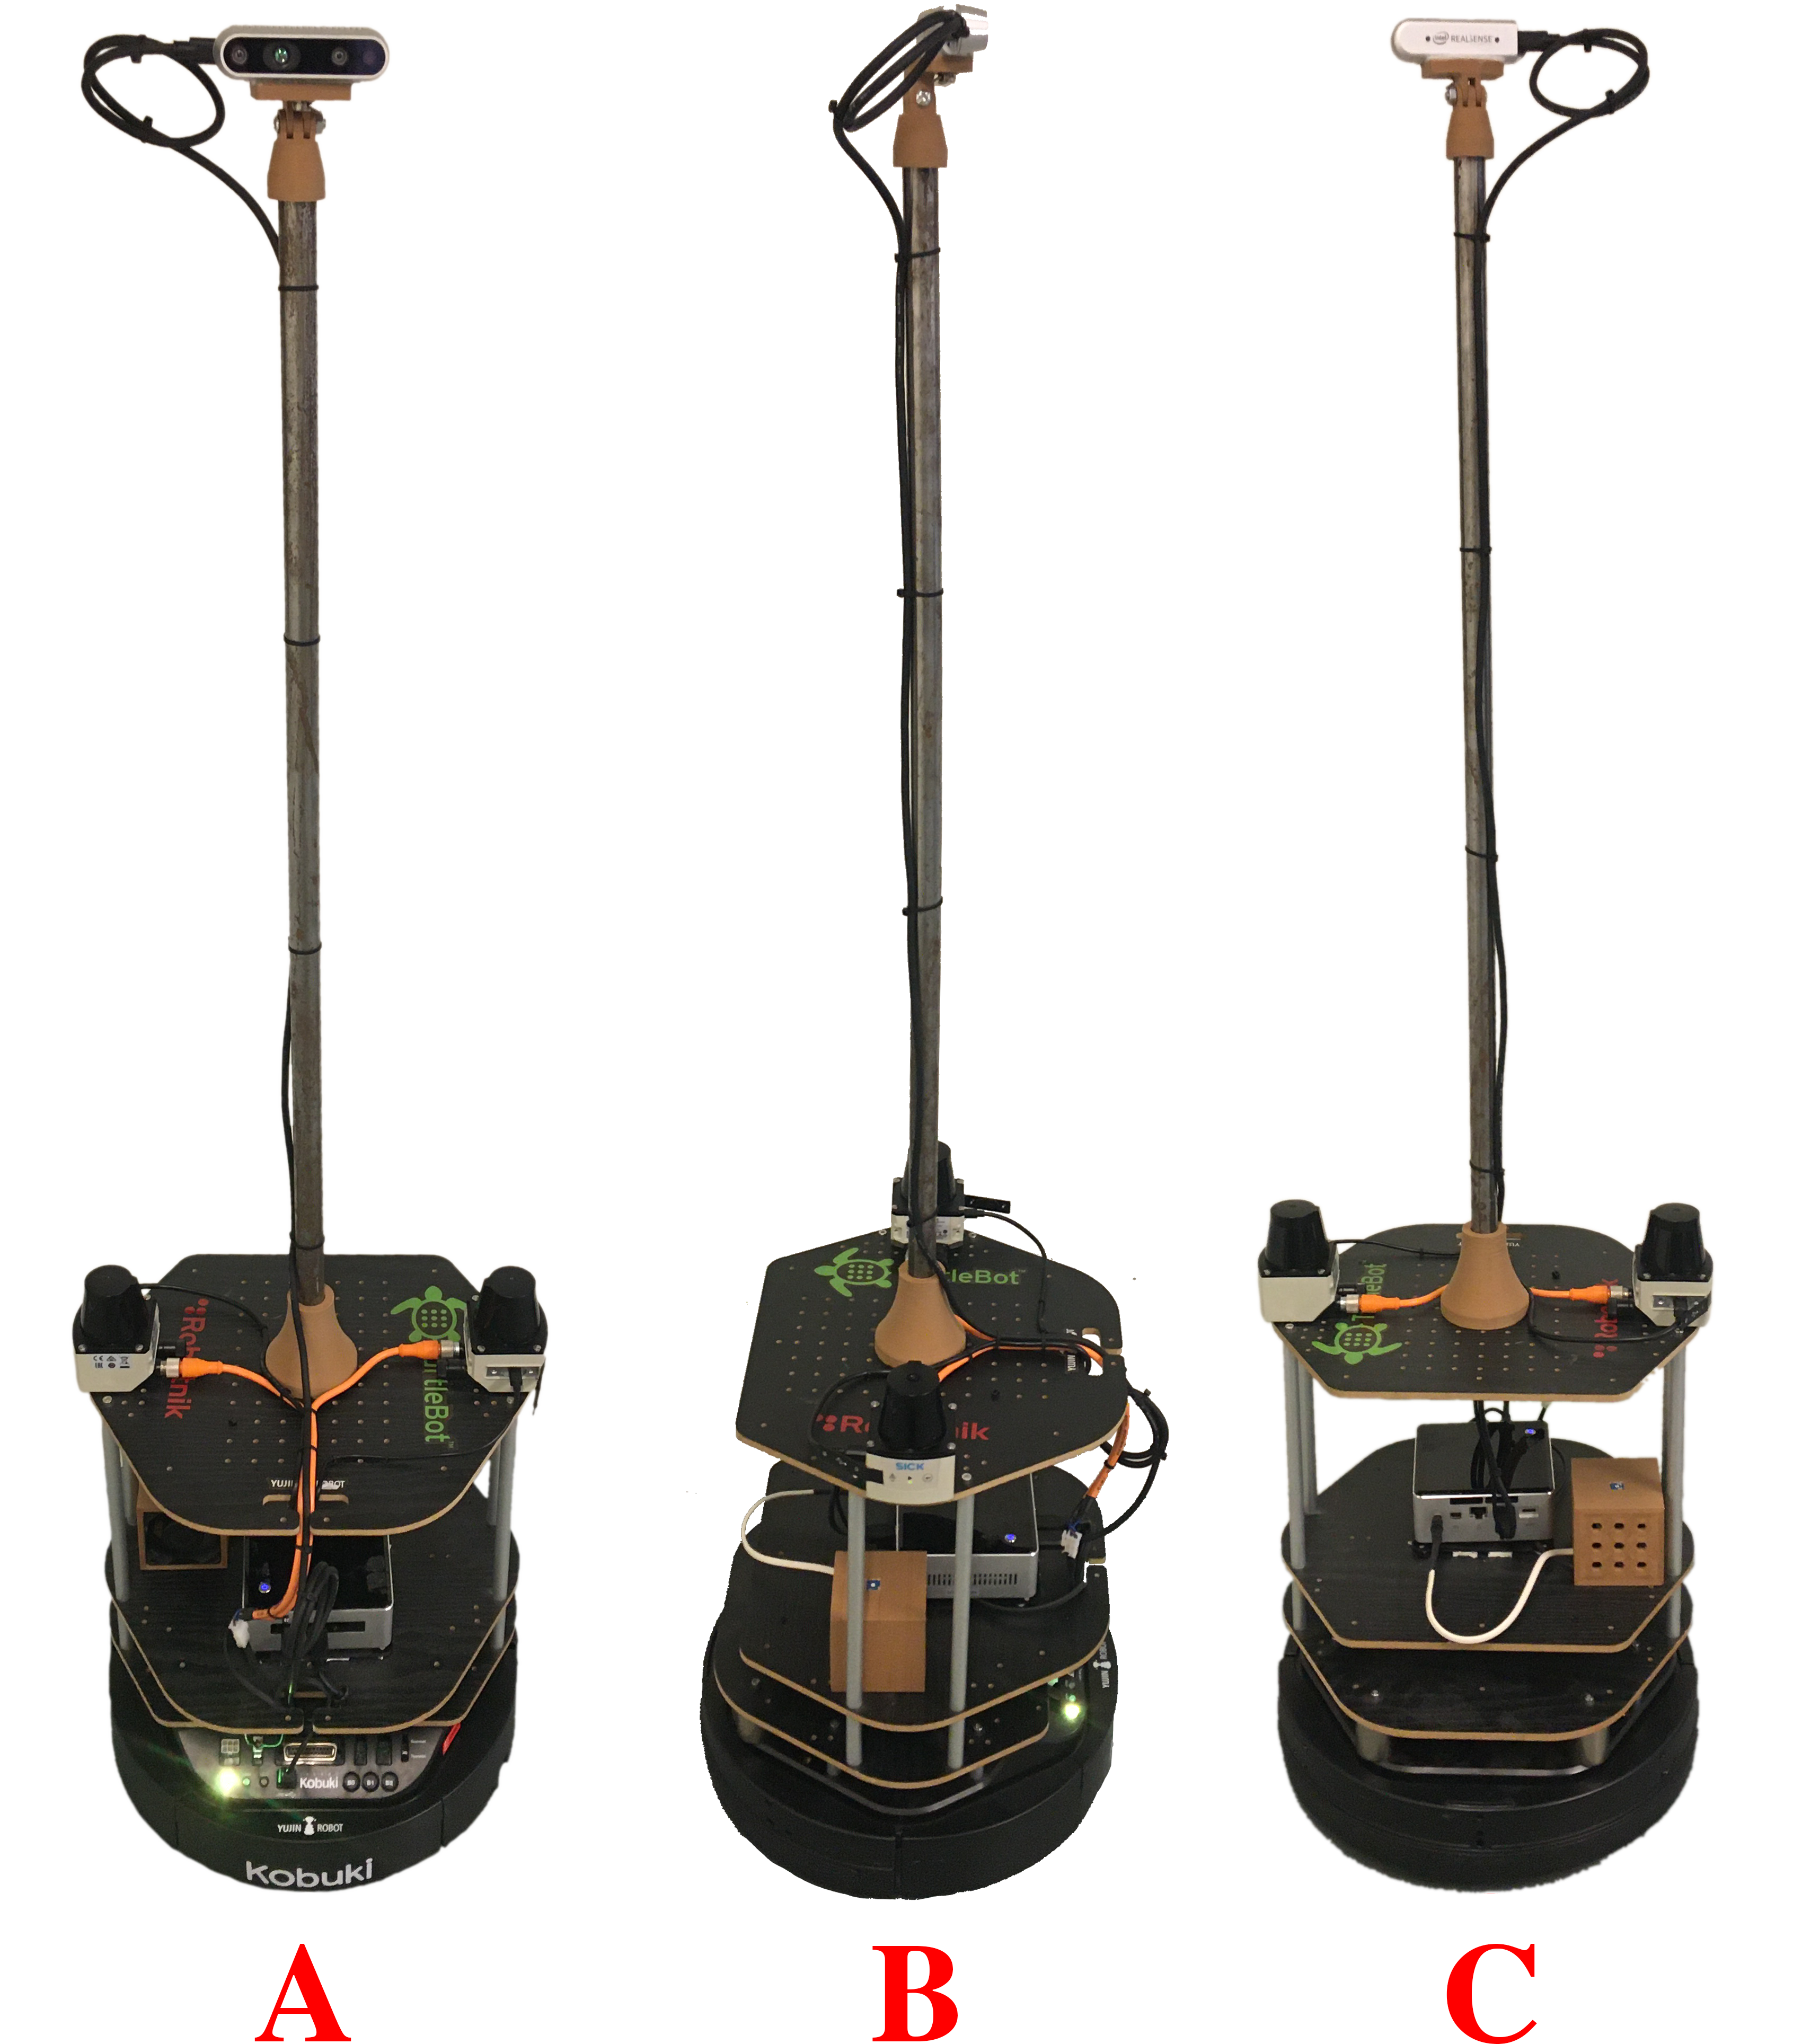
\includegraphics[width=.8\textwidth]{figures/TurtleBotFull.png}
    \caption{The physical prototype used for this project. A: The prototype seen from the back with the camera facing the user. B: The prototype seen from the side. C: The prototype seen from the front.}
    \label{fig:PhysicalSetup}
\end{figure}

The physical setup consists of the equipment previously described along with components to connect everything together. The main component for the connection of data streams from sensors is the NUC from intel. The NUC is a mini PC usable for many different purposes\cite{IntelNUC}. In this project the NUC is the main controller of the robot used to gather data from the sensors and do computations in order to determine the actions of the robot.\\

\begin{figure}[H]
    \centering
    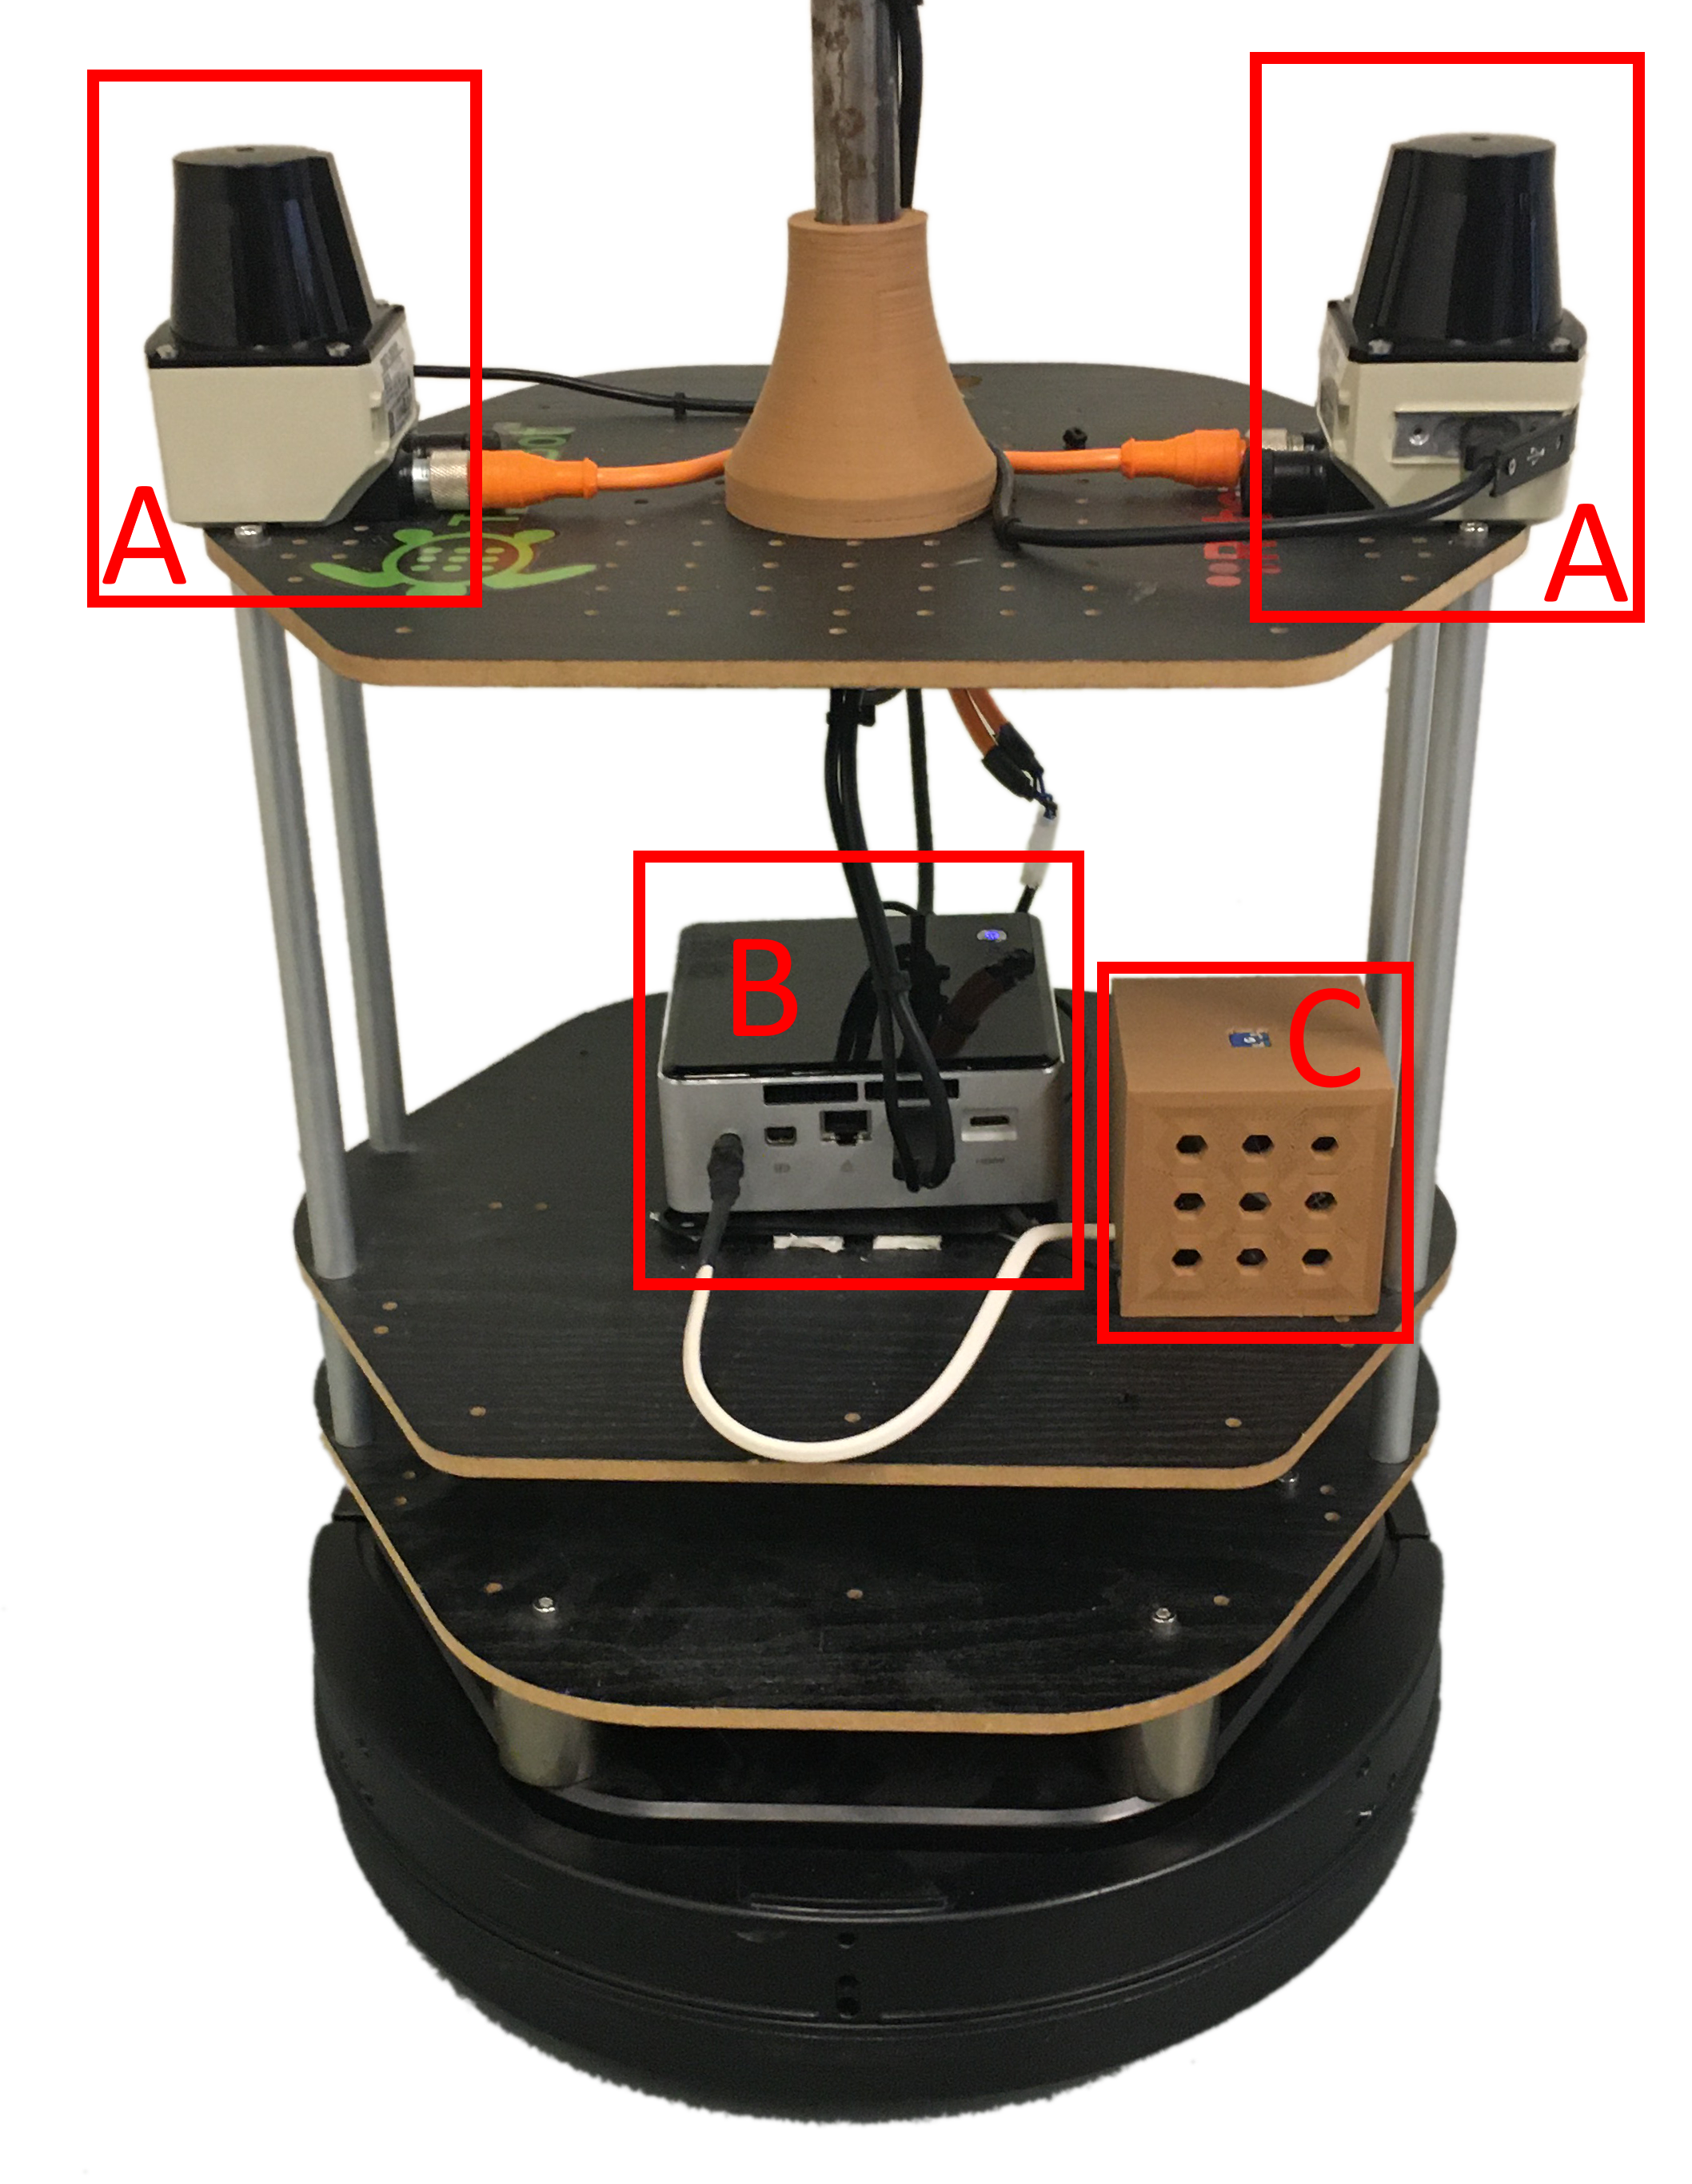
\includegraphics[width=.75\textwidth]{figures/Components.png}
    \caption{The components of the prototype. A: The SICK TIM571 LIDARS. B: The Intel NUC. C: Power convert for the Intel NUC.}
    \label{fig:Components}
\end{figure}

As can be seen in figure \ref{fig:Components}, the prototype carries all the needed components for this project. The LIDARS are placed on the top of the Turtlebot to be in the correct height for the leg detection, as described in section \ref{sec:height}. Additionally, the Intel Real Sense is mounted on a pole to put it in the correct height for facial detection as described in section \ref{sec:height}. In order to power the NUC from the Kobuki base, a power converter was made. This converter ensures that the NUC can run while the Kobuki base is turned on. Additionally, the battery level of the robot is monitored using one the LEDs of the Kobuki base. When the colour changes from green to yellow, the power is getting low. When the LED turns red the robot should be charged.\\